\section{The Quorum protocol}
The {\em Quorum} protocol is a consensus protocol proposed in~\cite{guerraoui2012speculative}
as complementary to the Paxos consensus protocol~\cite{gafni2003disk} under perfect
channel conditions. {\em Consensus} allows a set of communicating processes
(clients and servers in our case) to agree on a common value. Each of clients proposes
a value and receives a common decision value. The authors in~\cite{guerraoui2012speculative}
propose to use Quorum when no failures occur (perfect channel conditions) and 
Paxos when less than half of the servers may fail. 

The Quorum protocol operates as follows.
\begin{enumerate}
 \item Upon proposal, a client $c$ broadcasts its proposed value 
 $v$ to all servers. It also saves $v$ in its local memory and starts a local time
 $t_c$. 
 \item When a server receives a value $v$ from a client $c$, it performs
 the following check.
 \begin{itemize}
  \item It if has not sent any accept messages, it sends an accept message
  $accept(v)$ to the client $c$. 
  \item If it has already accepted value $v'$, it sends an accept message
  $accept(v')$ to the client $c$. 
 \end{itemize}
 \item If a client $c$ receives two different accept messages, it switches
 to the backup phase $switch-backup(proposal_c)$.
 \item If a client $c$ receives the same accept messages $accept(v)$ from all the servers,
 it decides on the value $v$.
 \item If a client's timer $t_c$ expires, it waits for at least
 one accept message $accept(v')$ from a server, or chooses a value $v'$
 from an already received $accept(v')$ message, and then switches to 
 the backup phase with the value $v'$. 
 \item The {\em backup} phase is an implementation of the Paxos algorithm. Quorum in this
 case has decided that the channel is not perfect. 
\end{enumerate}

We implemented the Quorum protocol in BIP, and we used \biptool{} to verify 
two invariants as defined in~\cite{guerraoui2012speculative}.
\begin{enumerate}
 \item[$Invariant_1$] If a client $c$ decides on a value $v$, then all clients 
 $c' \neq c$ that have switched, either before or after $c$, switch with the value $v$.
 \item[$Invarian_2$] If a client $c$ decides on a value $v$, then all clients
 $c' \neq c$ who decide, do so with the same value $v$. 
\end{enumerate}

Table~\ref{tb:bip:qrm} shows the results of using \biptool{} to verify the 
Quorum protocol for $2$ and $4$ clients with $2$ servers. The designs
are indexed as \cci{num\_clients}-\cci{num\_servers}-\cci{status} where 
\cci{num\_clients} is the number of clients, \cci{num\_servers} is the number of 
servers and \cci{status} is either valid (\cci{v}) or erroneous (\cci{e}).
A valid design contains no design bugs, while an errneous design is injected
with a bug. We report on the size of the AIG in terms of number of latches (\cci{lat}),
number of AND gates (\cci{and}) and logic levels (\cci{lev}) before and after
applying reduction algorithms. We also show the time taken by ABC to decide the problem, 
and the total time taken for reduction and decision procedures. 
A $\checkmark$ decision indicates that ABC proved that the property is never 
violated, \ie{} the design is valid, while a $\chi$ decision means that 
ABC was able to find a counter example that violates the property. 

\begin{table}[bt]
\caption{Quorum results}
\centering
\begin{tabular}{|c|c|c|c|c|c|c|c|c|c|}
\cline{2-9}
\multicolumn{1}{c|}{} & \multicolumn{ 3}{c|}{Original} & \multicolumn{ 3}{c|}{After reduction} & \multicolumn{ 2}{c|}{Time (s)} & \multicolumn{1}{l}{} \\ \hline
Design & lat & and & lev & lat & and & lev & Ver. & Tot. & Decision \\ \hline
2-2-v & 264 & 3614 & 105 & 66 & 641 & 29 & 240.6 & 245 & $\checkmark$\\ \hline
2-2-e & 264 & 3508 & 101 & 65 & 923 & 51 & 0.78 & 0.11 & $\chi$\\ \hline
4-2-v & 390 & 6453 & 151 & 117 & 1170 & 30 & \multicolumn{2}{c|}{58 hours}& $\checkmark$\\ \hline
4-2-e & 390 & 6305 & 145 & 117 & 1129 & 50 & 0.24 & 0.31 & $\chi$ \\ \hline
\end{tabular}
\label{tb:bip:qrm}
\end{table}

Using ABC's synthesis and reduction algorithms, \biptool{} was able to
reduce the size of the generated AIGs for all designs by a factor larger
than $50\%$. Furthermore,
\biptool{} was able to give conclusive results about all four designs, unlike
NuSMV which failed to give any decision about the designs having
$4$ clients and $2$ servers. For example, \biptool{} found a counter example for the erroneous 
design having $4$ clients and $2$ servers in $0.24 (s)$ while NuSMV failed to do
so. Figure~\ref{fig:res:counter} shows a snippet of the generated counter example for the 
erroneous design, visualized using the Gtkwave~\cite{bybell2010gtkwave} waveform viewer. 
The variables presented in the counterexample are the current control locations of
the different components in the design. 

\begin{figure}[bt]
\centering
\resizebox{1.0\textwidth}{0.25\textwidth}{
 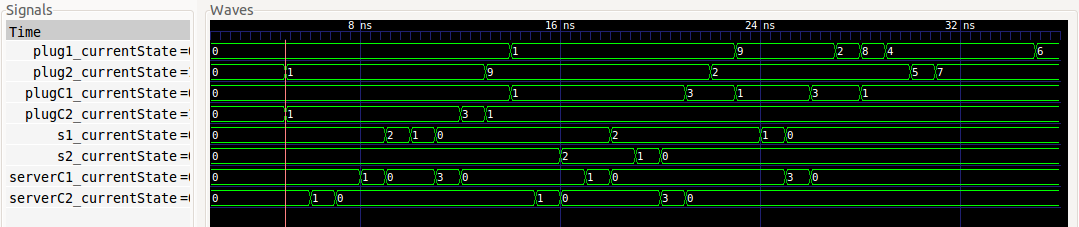
\includegraphics{figures/Quorum22CounterEx}
}
\caption{Visualization of a counter example using Gtkwave}
\label{fig:res:counter}
\end{figure}